\section{Model}
\label{sec:model}

\begin{comment}
Here you will present the architecture or model that you have chosen and which is implemented in your work.
Note that putting algorithms in your report is not always desirable, so in certain cases those might be placed in the appendix.
Code is normally to be avoided in the report itself, but may be included in an appendix or submitted as additional documents.
\textbf{(The actual code should also be submitted together with the report, either as a zip-file or as a link to a GitHub repository or similar.)}

Here, or in a separate section (or possibly in the Background section or in the Experimental Setup),
you should also discuss the data that you use in your experiments.

Clearly, a figure showing the architecture is a must, such as Figure~\ref{fig:Architecture}.

\begin{figure}[t!]
    \centering
    \missingfigure{Architecture figure to be added}
    \caption{The missing architecture}
    \label{fig:Architecture}
\end{figure}
\end{comment}

\begin{figure}
    \centering
    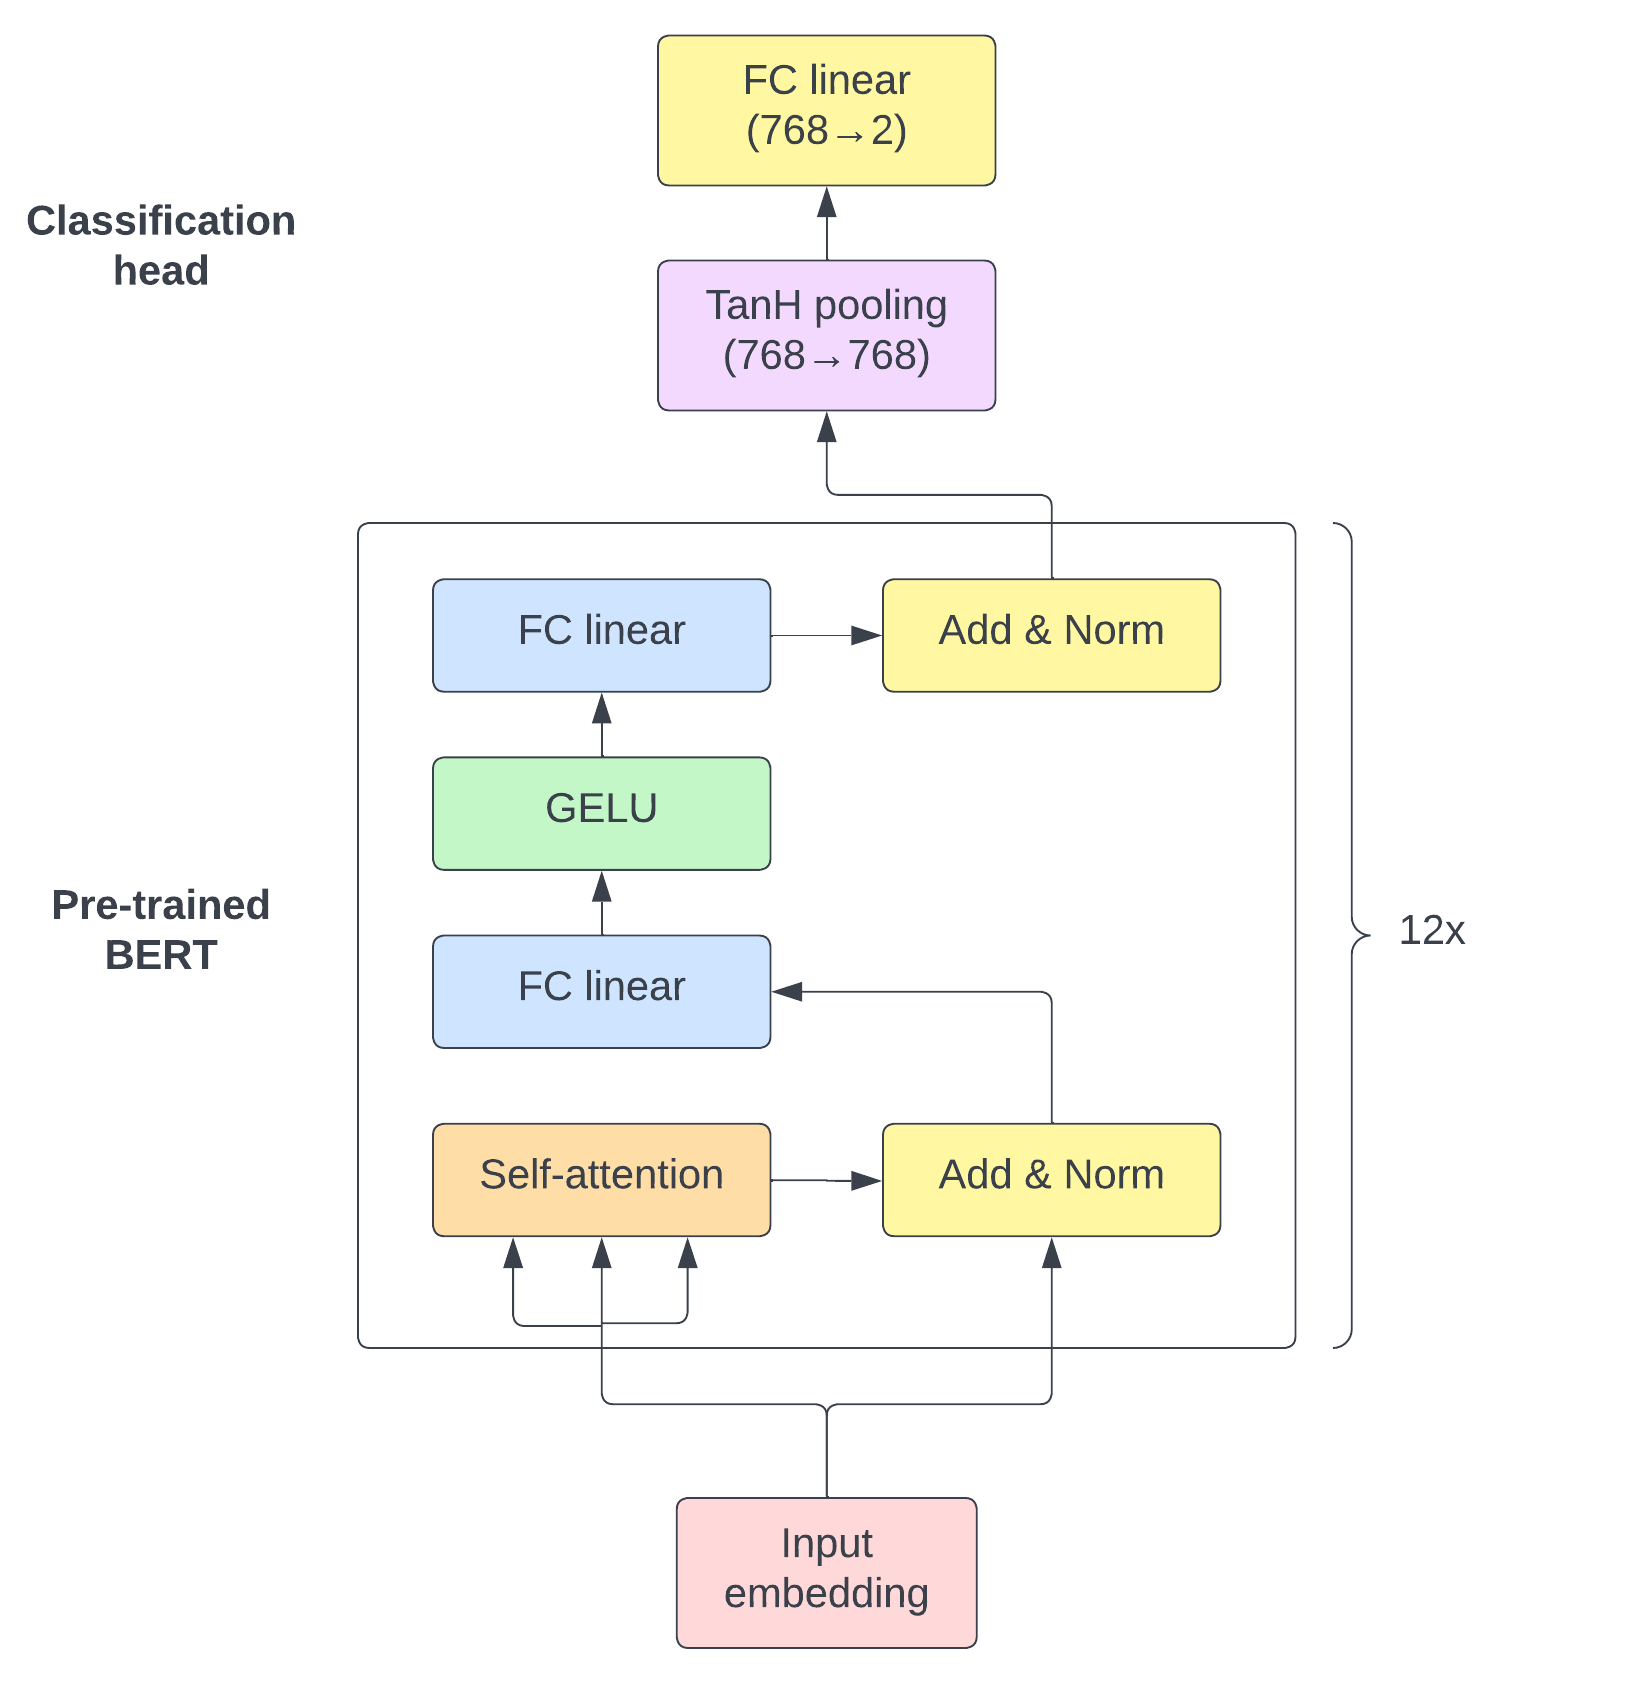
\includegraphics[width=0.7\textwidth]{figs/model_architecture.png}
    \caption{Model architecture}
    \label{fig:model-architecture}
\end{figure}

\autoref{fig:model-architecture} shows a rough model architecture. It consists of a pre-trained \acrshort{acr:bert} model with a classification head on top. This architecture is not representative for the \acrshort{acr:xmod}-based model used. The classification head has two outputs, namely  latitude and longitude coordinates. It takes as input the output corresponding to the \texttt{[CLS]} token, which captures the aggregated sequence representation. The hyperbolic tangent activation function adds some non-linearity to the output before it is fed into a fully connected linear layer, where latitude and longitude values are predicted.

Three different pre-trained models were tested in this project. These are \texttt{bert-base-german-uncased}\footnote{\url{https://huggingface.co/dbmdz/bert-base-german-uncased}}, \texttt{bert-base-german-cased-finetuned-swiss}\footnote{\url{https://huggingface.co/statworx/bert-base-german-cased-finetuned-swiss}}, and \texttt{ZurichNLP/swissbert}\footnote{\url{https://huggingface.co/ZurichNLP/swissbert}}. When selecting models, I was primarily interested in those trained on Swiss corpora, as this proved effective to \cite{scherrerHeLjuVarDial20202020}. \texttt{bert-base-german-uncased} is a German-language model pre-trained on a Wikipedia dump, EU Bookshop corpus, and more. \texttt{bert-base-german-cased-finetuned-swiss} is based on \texttt{bert-base-german-cased} and is pre-trained on the Leipzig Corpora Collection \citep{goldhahnBuildingLargeMonolingual} and SwissCrawl \citep{linderAutomaticCreationText2020}. \texttt{ZurichNLP/swissbert} is the only non-\acrshort{acr:bert} model used. It is based on \acrshort{acr:xmod}, with adapters trained for German, French, Italian, and Romansh Grishun.

Pre-trained models where accessed through Huggingface's \texttt{transformers} library.

% \begin{table}
%     \centering
%     \begin{tabular}{l|r}
%         \toprule
%         Model Name                                               & Model Type          \\
%         \midrule
%         dbmdz/\textbf{bert-base-german-uncased}                  & \acrshort{acr:bert} \\
%         statworx/\textbf{bert-base-german-cased-finetuned-swiss} & \acrshort{acr:bert} \\
%         ZurichNLP/\textbf{swissbert}                             & \acrshort{acr:xmod} \\
%         % ZurichNLP/\textbf{swissbert-xlm-vocab}            & \acrshort{acr:xmod} \\
%         \bottomrule
%     \end{tabular}
%     \caption{Pre-trained models used in the project}
%     \label{tbl:models-used}
% \end{table}

